\documentclass[tikz,border=8pt]{standalone}
\usepackage[T1]{fontenc}
\usepackage{xcolor}
\usepackage{helvet}
\usepackage{tikz}
\usetikzlibrary{arrows.meta,calc,shadows}
% ---- publication palette ----
\definecolor{resink}{RGB}{26,34,44}
\definecolor{resmuted}{RGB}{97,108,122}
\definecolor{reshair}{RGB}{214,220,228}
\definecolor{resnavy}{RGB}{31,78,121}
\definecolor{resnavysoft}{RGB}{238,244,250}
\definecolor{resgreen}{RGB}{42,117,91}
\definecolor{resred}{RGB}{150,40,40}
\definecolor{resamber}{RGB}{184,106,27}

\newcommand{\resfsTitle}{\sffamily\fontsize{9.4}{11}\selectfont\bfseries}
\newcommand{\resfsSub}{\sffamily\fontsize{6.7}{8.3}\selectfont}
\newcommand{\resfsCardT}{\sffamily\fontsize{7.6}{9}\selectfont\bfseries}
\newcommand{\resfsCardS}{\sffamily\fontsize{6.6}{8}\selectfont}
\newcommand{\resfsPill}{\sffamily\fontsize{5.9}{6.6}\selectfont\bfseries}
\newcommand{\resfsTiny}{\sffamily\fontsize{6.2}{7}\selectfont}

% proportion 0..1 -> x mm over plot band -70..30
\newcommand{\resX}[1]{-70+100*(#1)}

\newcommand{\rescard}[6]{%
	\pgfmathsetmacro{\resch}{#1-#2}\pgfmathsetmacro{\rescy}{(#1+#2)/2}
	\node[rectangle, rounded corners=5pt, fill=white, draw=reshair, line width=0.7pt,
	minimum width=212mm, minimum height=\resch mm, inner sep=0pt,
	drop shadow={shadow xshift=0.7pt, shadow yshift=-1pt, opacity=0.09, fill=black}]
	at (0,\rescy) {};
	\begin{scope}
		\clip[rounded corners=5pt] (-106,#2) rectangle (106,#1);
		\shade[left color=#3, right color=#3!35] (-106,#1-1.1) rectangle (106,#1);
	\end{scope}
	\draw[reshair, rounded corners=5pt, line width=0.7pt] (-106,#2) rectangle (106,#1);
	\node[rounded corners=2.5pt, fill=resink, text=white, minimum width=7.5mm,
	minimum height=5mm, inner sep=0pt, font=\sffamily\fontsize{6.8}{8}\selectfont\bfseries]
	at (-97.75,#1-5.5) {#4};
	\node[anchor=west, text=resink, font=\resfsTitle] at (-92.5,#1-5.5) {#5};
	\node[anchor=north west, text=resmuted, font=\resfsSub] at (-101.5,#1-9.3) {#6};
	\draw[reshair, line width=0.6pt] (-101.5,#1-13.5) -- (101.5,#1-13.5);
}

\newcommand{\respill}[5]{%
	\node[anchor=#4, rounded corners=2.2pt, fill=#1!11, text=#1!85!black,
	inner xsep=3pt, inner ysep=1.5pt, font=\resfsPill] at (#2,#3) {#5};}

\newcommand{\resrowlab}[4]{%
	\draw[#2, line width=1.5pt, line cap=round] (-100.6,#1-3.3) -- (-100.6,#1+3.3);
	\node[anchor=west, text=resink, font=\resfsCardT] at (-98,#1+1.9) {#3};
	\node[anchor=west, text=resmuted, font=\resfsCardS] at (-98,#1-2.1) {#4};}

\newcommand{\reswhisk}[4]{%
	\draw[resnavy, line width=#4, line cap=butt] ({\resX{#2}},#1) -- ({\resX{#3}},#1);
	\draw[resnavy, line width=0.7pt, line cap=butt] ({\resX{#2}},#1-1.3) -- ({\resX{#2}},#1+1.3);
	\draw[resnavy, line width=0.7pt, line cap=butt] ({\resX{#3}},#1-1.3) -- ({\resX{#3}},#1+1.3);}
\newcommand{\resdot}[2]{\draw[white, line width=0.5pt, fill=resnavy] ({\resX{#2}},#1) circle (1.25);}
\newcommand{\resvals}[4]{%
	\node[anchor=west, text=resink, font=\resfsCardT, inner sep=0pt] at (36,#1) {#2};
	\node[anchor=west, text=resmuted, font=\resfsCardS, inner sep=0pt] at (62,#1) {[#3,\,#4]};}

\newcommand{\resgrid}[2]{%
	\foreach \v in {0,0.25,0.5,0.75,1} {\draw[reshair, line width=0.5pt] ({\resX{\v}},#1) -- ({\resX{\v}},#2);}
	\draw[resmuted!55, line width=0.6pt] ({\resX{0}},#2) -- ({\resX{1}},#2);
	\foreach \v/\lab in {0/{0},0.25/{25},0.5/{50},0.75/{75},1/{100}}
	{\node[anchor=north, text=resmuted, font=\resfsTiny, inner sep=1pt] at ({\resX{\v}},#2-0.9) {\lab};}
}

\begin{document}
	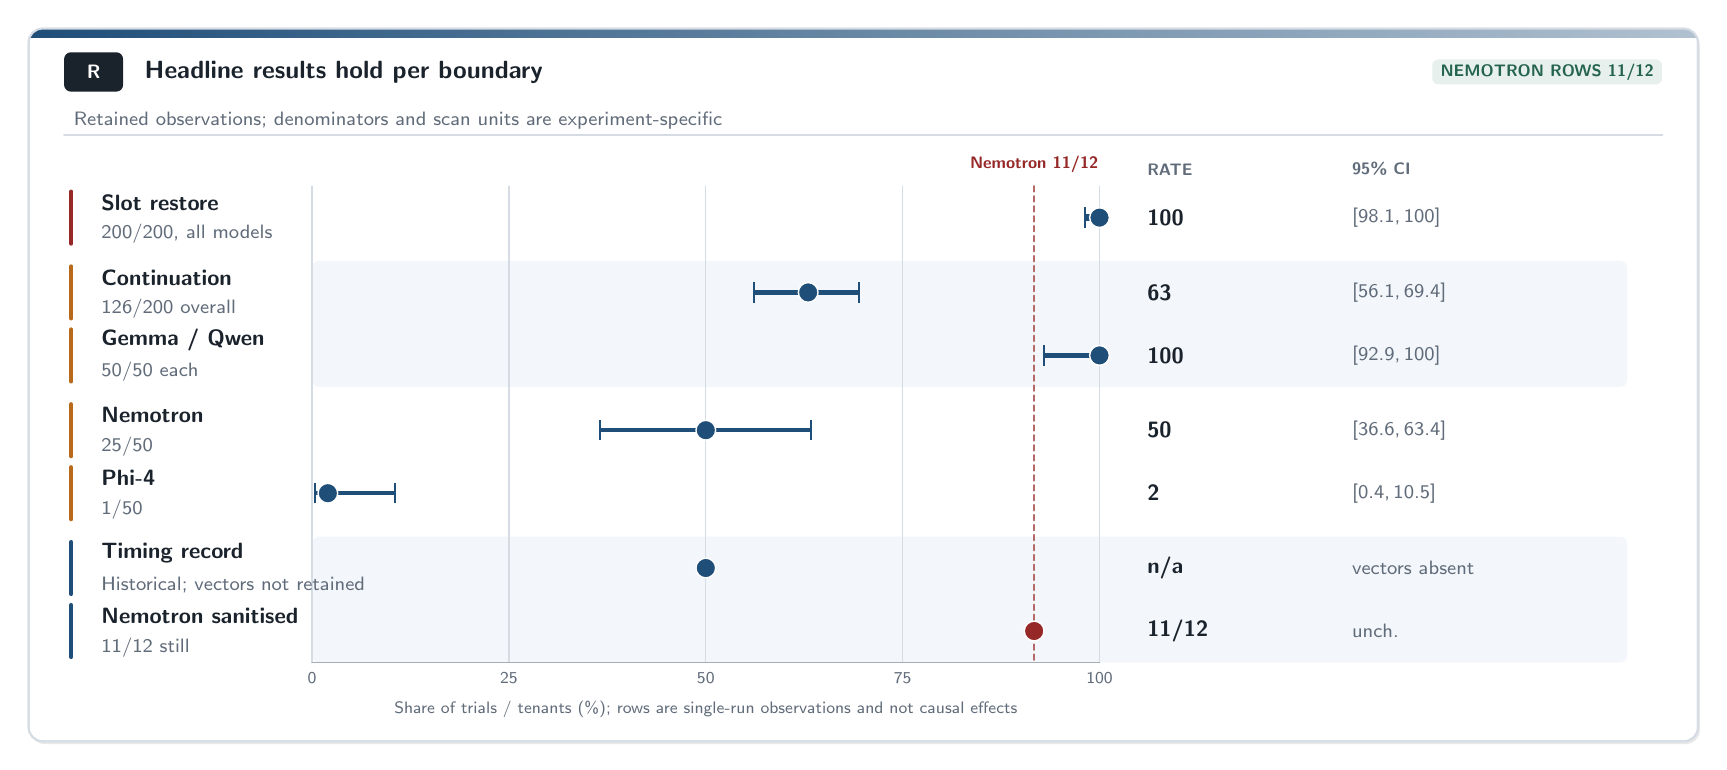
\begin{tikzpicture}[x=1mm,y=1mm,>=Latex,line cap=round,line join=round,font=\sffamily]

		\rescard{40}{-50.5}{resnavy}{R}{Headline results hold per boundary}
		{Retained observations; denominators and scan units are experiment-specific}
		\respill{resgreen}{101.5}{34.5}{east}{NEMOTRON ROWS 11/12}

		\fill[resnavysoft!70, rounded corners=2.5pt] (-70,10.5) rectangle (97,-5.5);
		\fill[resnavysoft!70, rounded corners=2.5pt] (-70,-24.5) rectangle (97,-40.5);
		\resgrid{20}{-40.5}

		% combined tenant band (unchanged): shade 11/12 region marker
		\draw[resred!70, dash pattern=on 2pt off 1.6pt, line width=0.7pt] ({\resX{0.917}},20) -- ({\resX{0.917}},-40.5);
		\node[anchor=south, text=resred, font=\resfsTiny\bfseries, inner sep=1pt] at ({\resX{0.917}},21.3) {Nemotron 11/12};

		\node[anchor=south west, text=resmuted, font=\resfsTiny\bfseries, inner sep=0pt] at (36,21.3) {RATE};
		\node[anchor=south west, text=resmuted, font=\resfsTiny\bfseries, inner sep=0pt] at (62,21.3) {95\% CI};

		\resrowlab{16}{resred}{Slot restore}{200/200, all models}
		\resrowlab{6.5}{resamber}{Continuation}{126/200 overall}
		\resrowlab{-1.5}{resamber}{Gemma / Qwen}{50/50 each}
		\resrowlab{-11}{resamber}{Nemotron}{25/50}
		\resrowlab{-19}{resamber}{Phi-4}{1/50}
		\resrowlab{-28.5}{resnavy}{Timing record}{Historical; vectors not retained}
		\resrowlab{-36.5}{resnavy}{Nemotron sanitised}{11/12 still}

		\reswhisk{16}{0.981}{1.0}{2.4pt}
		\reswhisk{6.5}{0.561}{0.694}{1.6pt}
		\reswhisk{-1.5}{0.929}{1.0}{1.6pt}
		\reswhisk{-11}{0.366}{0.634}{1.6pt}
		\reswhisk{-19}{0.004}{0.105}{1.6pt}
		\resdot{16}{1.0}\resdot{6.5}{0.63}\resdot{-1.5}{1.0}\resdot{-11}{0.5}\resdot{-19}{0.02}
		% timing + sanitised rows are descriptive markers
		\draw[white, line width=0.5pt, fill=resnavy] ({\resX{0.5}},-28.5) circle (1.25);
		\draw[white, line width=0.5pt, fill=resred] ({\resX{0.917}},-36.5) circle (1.25);

		\resvals{16}{100}{98.1}{100}
		\resvals{6.5}{63}{56.1}{69.4}
		\resvals{-1.5}{100}{92.9}{100}
		\resvals{-11}{50}{36.6}{63.4}
		\resvals{-19}{2}{0.4}{10.5}
	\node[anchor=west, text=resink, font=\resfsCardT, inner sep=0pt] at (36,-28.5) {n/a};
	\node[anchor=west, text=resmuted, font=\resfsCardS, inner sep=0pt] at (62,-28.5) {vectors absent};
	\node[anchor=west, text=resink, font=\resfsCardT, inner sep=0pt] at (36,-36.5) {11/12};
		\node[anchor=west, text=resmuted, font=\resfsCardS, inner sep=0pt] at (62,-36.5) {unch.};

		\node[text=resmuted, font=\resfsTiny] at ({\resX{0.5}},-46.5)
		{Share of trials / tenants (\%); rows are single-run observations and not causal effects};

	\end{tikzpicture}
\end{document}
